\textit{Introduce topic by talking about cells. Attention grabber, relate biophysics study to cancer reserach and many areas where we need to focus our research. Short and sweet, maybe 1 or 2 short paragraphs.}

	Neurodegenerative diseases, such as Alzheimer's and Huntinton's disease, have consistently been one of the leading causes of death in the United States. Scientists all over the world struggle to find the leading causes of these diseases and continue to hope for a breakthrough in science in attempt to prevent or even cure these fatal diseases. Although this breakthrough has yet to come, research suggests that motor protein failure is a main cause of cell degeneration. More specifically, defects in the motor protein dynein has been linked to neurodegeneration due to the cell's funtional dependence on dynein and its mechanical properties. However, unlike dynein's motor protein siblings, dynein possesses a unique structure causing it to stochasitcally move around the cell and be unpredicatable in nature. Thus, fully understanding the mechanisms of dynein can allow us to further conclude causes of its failure, putting us one step closer to discovering the major breakthrough for neurodegenerative research. In this paper, we propose a model of dynein that uses Monte Carlo methods and a Brownian dynamics simulation in order to reproduce the steping behavior observed from experiment. that reproduces the stepping behavior of experiment using Monte Carlo methods and a Brownian dynamics simulation.  

\section{Background}

\begin{figure}[H]
	\centering
	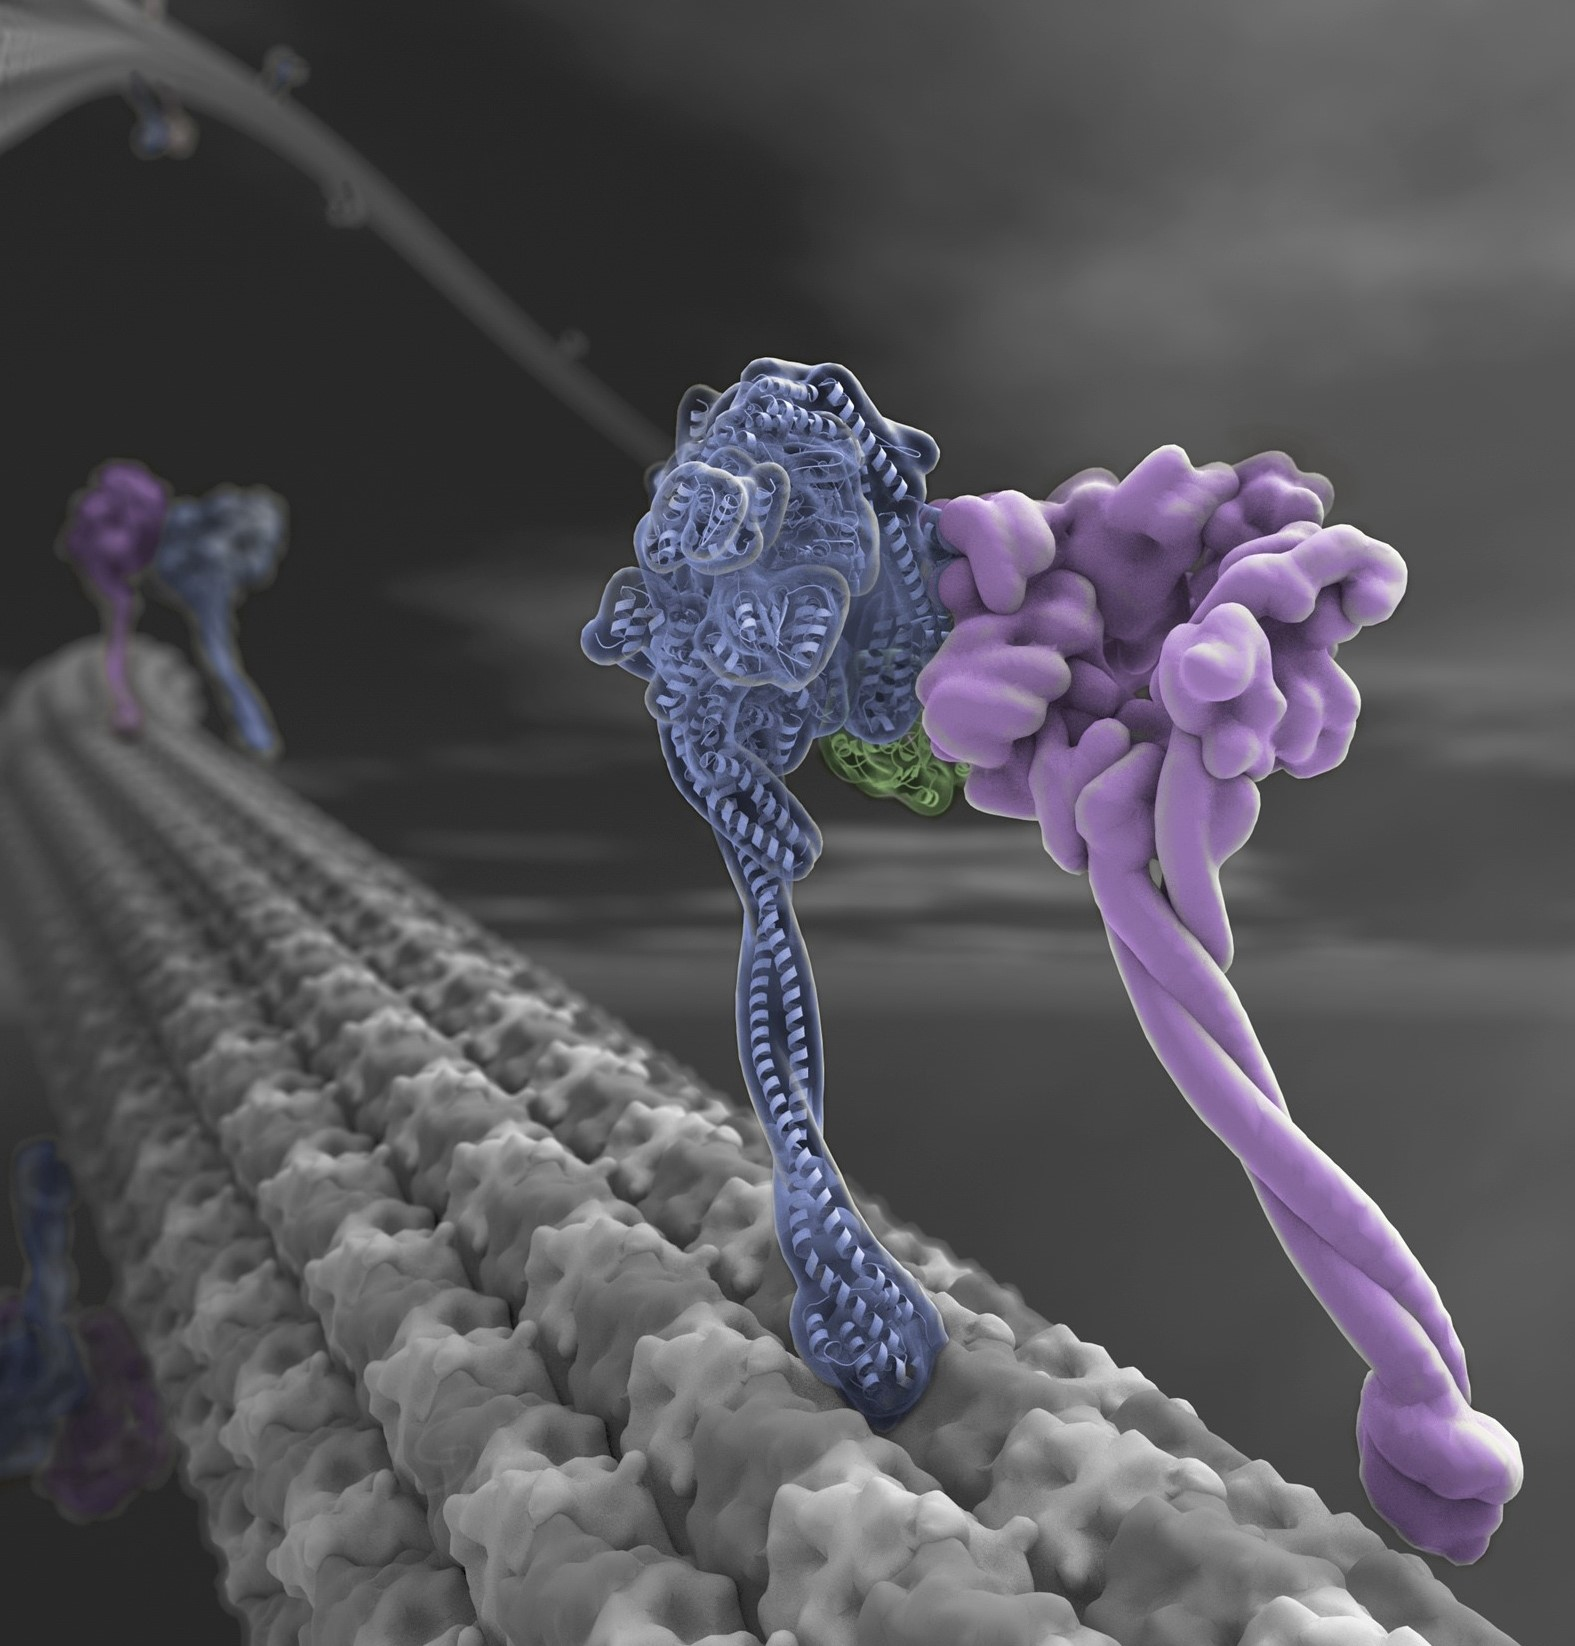
\includegraphics[width=0.5\columnwidth]{Figures/dynein_walking_art.jpg}
	\caption[Artist Rendition of Dynein]{\textbf{Artist Rendition of Dynein} \cite{JohnsonArt}}
	\label{fig:ArtDynein}
\end{figure}

Cells are complicated. Despite their fatal degeneracies, cells have the ability to move, perfectly divide, and spatially organize themselves. They can do so because tiny, two-legged molecular proteins, named \textit{motor proteins}, carry cargo containing information that outlines the blueprint for different functions within the cell. These motor proteins consists of kinesin, myosin, and dynein. They can travel all around the cell on a cytoskeleton composed of microtubules (MT) that act as a walkway for the proteins. A depiction of dynein walking along the microtubule is shown above in Figure (\ref{fig:ArtDynein}). Microtubules are constructed from negatively charged $\alpha$ and positively charged $\beta$ tubulin dimers that polarizes the microtubule depending on which tubulin is left hanging at the ends. In a eukaryotic cell, microtubules typically stem outwards from the cell's nucleus to the cell walls where the $\beta$ tubulin is exposed, generating a positive end that pulls kinesin and myosin. However, dynein opposes kinesin and myosin by walking towards the nucleus cell body where the MT is negatively charged. This attraction to both ends drives the directed stepping motion for each motor protein and is shown in Figure (\ref{fig:transport}). 

\begin{figure}[H]
	\centering
	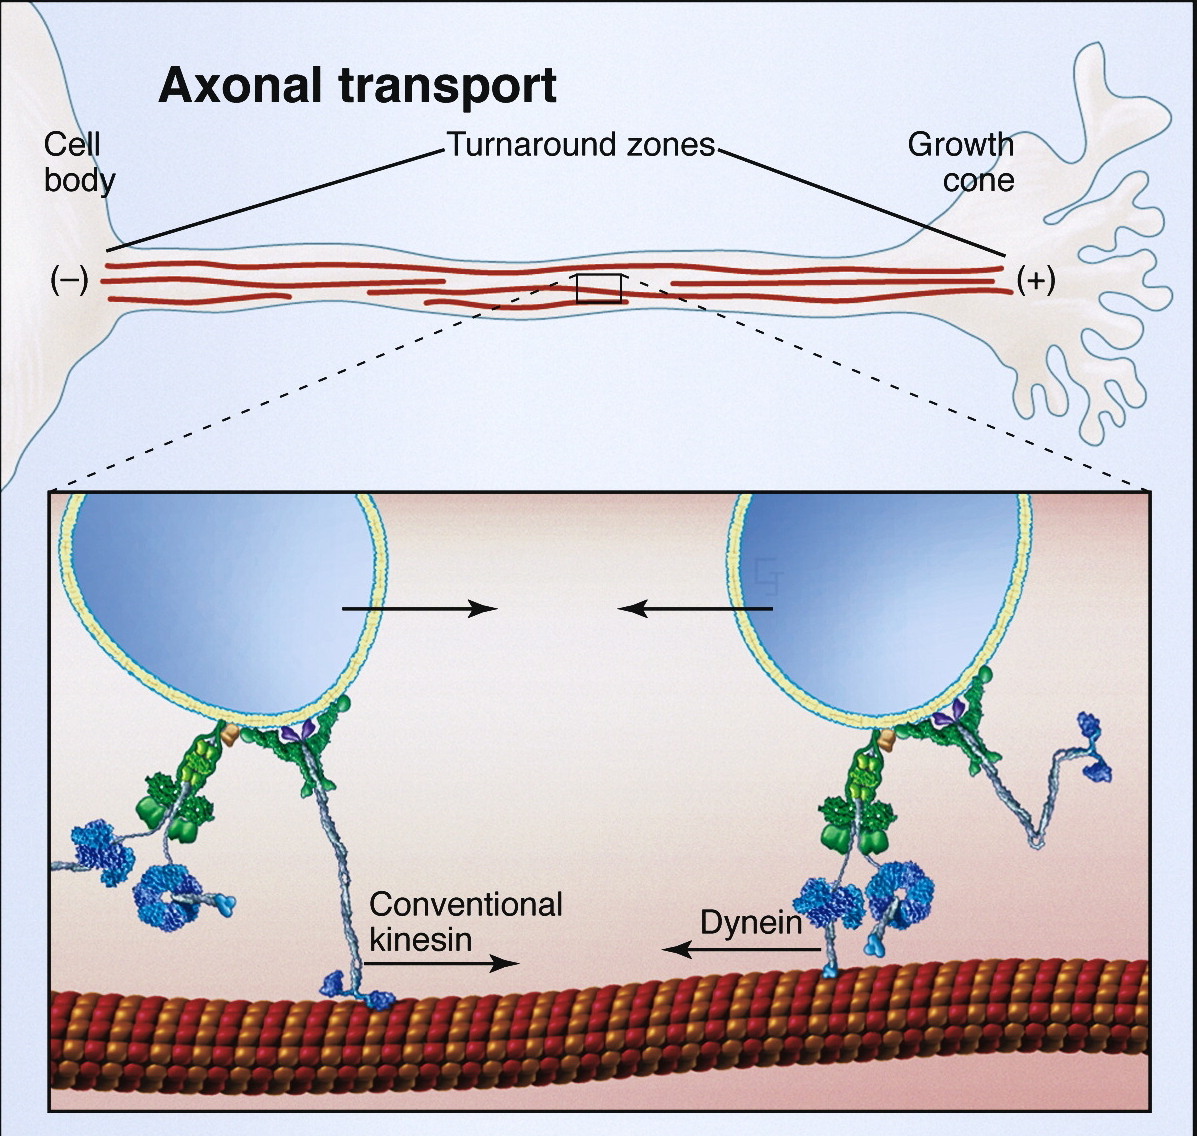
\includegraphics[width=0.6\columnwidth]{Figures/retrograde_transport.jpg}
	\caption[Retrograde Transport]{\textbf{Retrograde Transport} \cite{Vale2003molecular}}
	\label{fig:transport}
\end{figure}

Both kinesin and myosin exhibit hand-over-hand stepping, where their ``legs" take turns alternating steps like a human. Due to dynein's massive size compared to its motor protein siblings, dynein does not step uniformly but rather inchworms its ``feet" like a drunk human. This unique property makes dynein difficult to study when analyzing possible sources of molecular failure, but utters the importance of understanding the physical structure of the entire motor protein.

\section{Structure}
\textit{In-detail background knowledge on structure of dynein. Talk about each domain and their roles. Binding domain, six AAA+ domains, tail, and cargo. Stalk and linker that attaches things together. How the structure is so much larger than that of kinesin. dynein has flexibility because of its linker and in order to compensate for its huge domains. }

Dynein is composed of two motor heavy chain subunits of linked amino acids, called polypeptides, each which are separated into domains. These domains are the tail domain, the six AAA+ domains (which creates a ring and is often called the motor domain), and the microtubule binding domains, where a linker connects the tail to the AAA+ ring and a stalk connects the AAA+ ring to the binding domain. Figure (\ref{fig:structure}) displays a simplified dynein where both subunits are connected to the tail with separate linkers. 

%\begin{figure}[H]
%	\centering
%	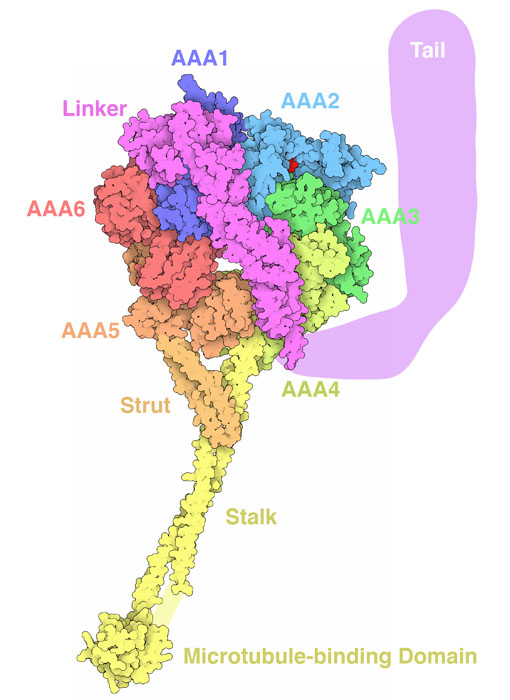
\includegraphics[width=0.6\columnwidth]{Figures/dynein_polypeptide.jpg}
%	\caption[Polypeptide Structure]{\textbf{Polypeptide Structure} \cite{GoodsellArt}}
%	\label{fig:polypeptide}
%\end{figure}

\begin{figure}[H]
	\centering
	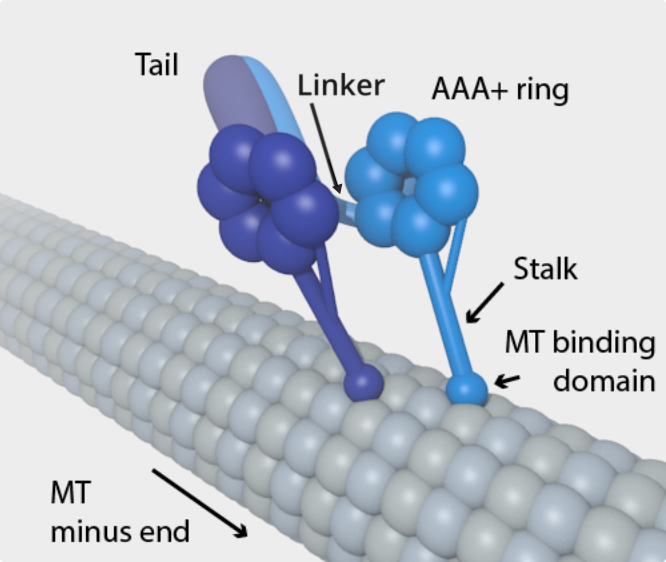
\includegraphics[width=0.6\columnwidth]{Figures/dynein_on_MT.png}
	\caption[Dynein on Microtubule]{\textbf{Dynein on Microtubule} Artist’s illustration of a dimer of cytoplasmic dynein heavy chains bounded to microtubule. This rendition similarly illustrates dynein’s structure as a domain-rod system. \cite{TheTrappistArt}}
	\label{fig:structure}
\end{figure}

Dynein's crystal structure has been intensely studied because of the pivotal role it plays in dyneins unpredictable stepping nature. Its inability to step uniformly is largely due to the large lengths between each major domain site, as the linker and stalk are about a factor of a half larger than the diameter of the AAA+ ring. This is unique when commpared to kinesin and myosin, as their motor domains are much closer to the MT causing their center of mass to keep the protein controlled and steady when stepping. Despite dynein's large structure, dynein can still achieve processive stepping towards the negative end of the MT by the interaction of ATP with the AAA+ domains, thus is why the AAA+ domains are referred to as the motor domains.





\section{Stepping}
\textit{Biology and chemistry of stepping. What is actually causing it to step? ATP hydrolysis. Maybe short introduction on stepping and go more in detail in Power Stroke model. Say there are multiple theories and models of how dynein steps. Powerstroke, Winch, etc. Power stroke is most accepted. It can step on microtubule that is made up of tubulin dimers, $\alpha$ and $\beta$ tubulins. They are normally 8nm apart and so experimentalists believe dynein average step is always factor of 8nm. }

Dynein's ability to step is entirely ATP driven under the process of ATP hydrolysis with its motor domains. 

\begin{figure}[H]
	\centering
	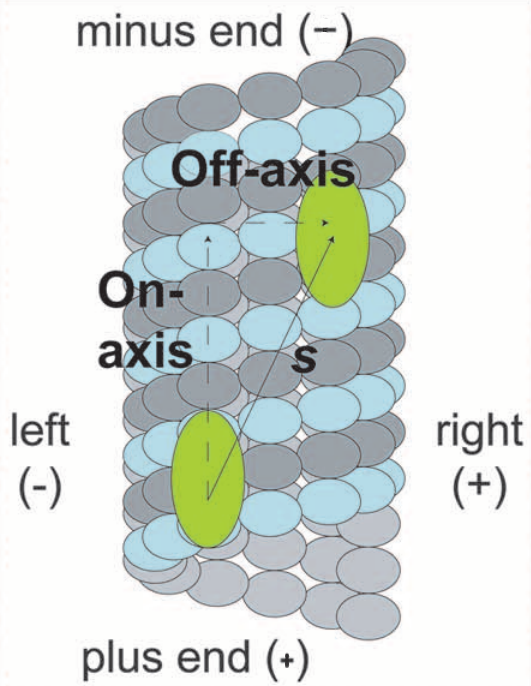
\includegraphics[width=0.3\columnwidth]{Figures/Onaxis.png}
	\caption[Stepping Axis]{\textbf{Stepping axis}  \cite{Dewitt2012} }
	\label{fig:YildizCorrelation}
\end{figure}

\textit{THIS IS STRAIGHT FROM PROPOSAL, NEED TO FIX THIS AND ADJUST SO THAT MORE DYNEIN DETAILS GOES INTO CHAPTER 2}

In a eukaryotic cell, dynein is one of the three motor proteins that are responsible for the cell’s ability to move, divide, and spatially organize itself. Similar to the more researched kinesin, dynein conveys cargo along the microtubule track by using ATP to power its two binding domains (its “feet”). However, its walking-like movements along the track are very unpredictable and can vary in terms of distance and direction. Dynein’s two feet can also act independently from each other causing much more erratic and stochastic steps. However, despite dynein’s stochastic nature, dynein is still able to achieve processive motion due to the functions of its structure. Structurally, dynein is composed of two motor heavy chain subunits of linked amino acids, called polypeptides, each which are separated into domains. These domains are the tail domain, the linker domain, the six AAA+ domains, and the microtubule binding domains (See Figure 1). The AAA+ domains are responsible for ATP hydrolysis, in which converts chemical energy stored in ATP into mechanical work causing dynein’s motility. 

Because dynein’s stepping is unpredictable in nature, its stepping mechanism has not been intensely studied as compared to its structure. Questions regarding the electrostatic interactions with the microtubule, ring stacking, discrete microtubule binding sites, or elasticity of the stalk are yet to be answered. A known and supported model to describe dynein’s motion is the powerstroke model, where ATP binding to an AAA+ domain triggers conformational changes that lowers the affinity of the binding domain for the microtubule, causing it to unbind and take a step . While the powerstroke model and other theorized stepping models exists, there are no such studies which use molecular dynamics to verify if these theorized mechanisms are feasible for the dynein motor to produce. There are studies that incorporate a computational model of dynein, but many use chemical rate transitions and assume independence of steps without simulating the precise protein dynamics within its step.




\subsection{Powerstroke Model}
\textit{Theorized model of stepping. Mechanochemical Cycle. Talk about ATP hydrolysis. Different conformational changes within a step. Look at linker and how it changes angles. Physically, it looks like it unbinds, stretches leg, then kicks forward, then diffuse back to MT.} 

\begin{figure}[H]
	\centering
	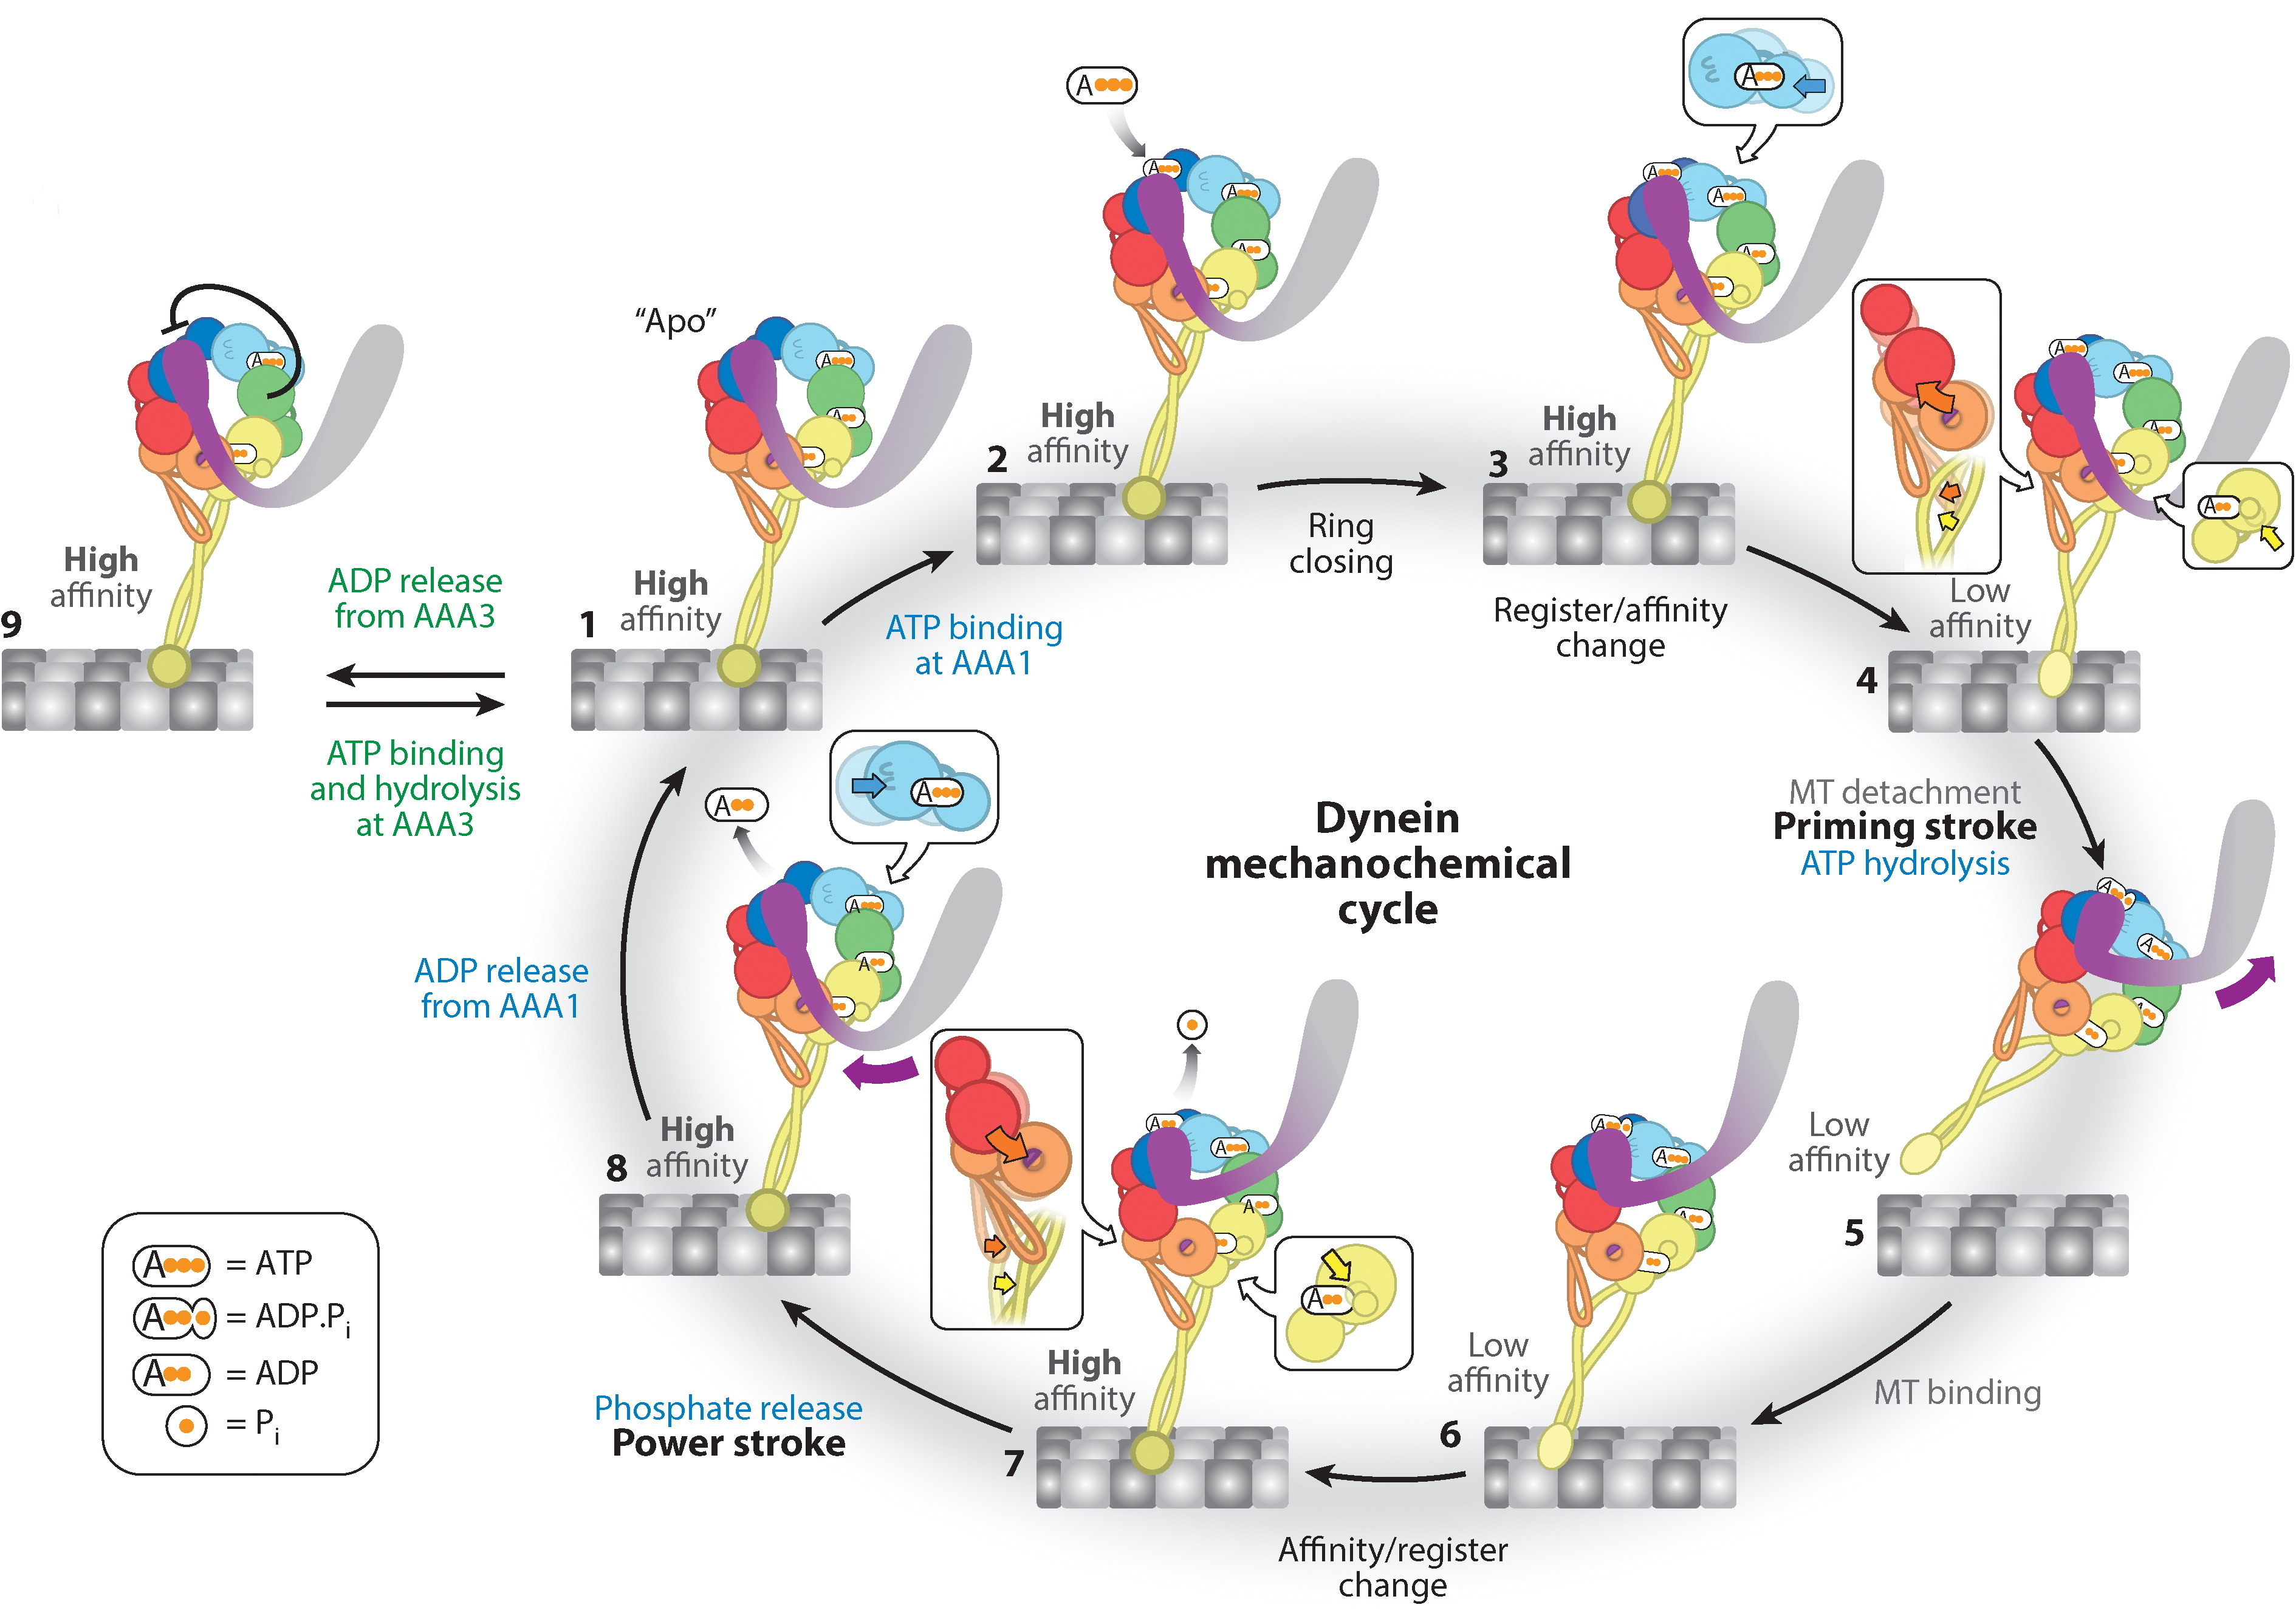
\includegraphics[width=1\columnwidth]{Figures/mechanochemical_cycle.jpeg}
	\caption[Mechanochemical Cycle]{\textbf{Mechanochemical Cycle}  \cite{Cianfrocco2015mechanism}}
	\label{fig:MechanochemicalCycle}
\end{figure}

\begin{figure}[H]
	\centering
	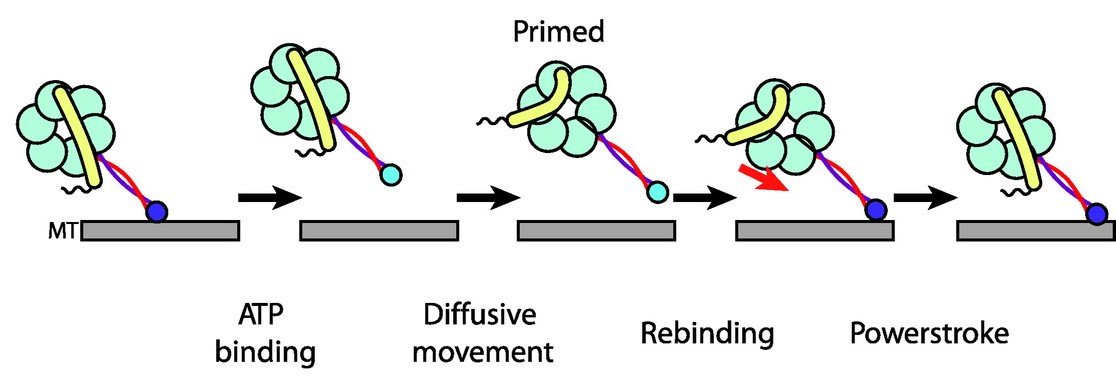
\includegraphics[width=1\columnwidth]{Figures/powerstroke.jpeg}
	\caption[Powerstroke]{\textbf{Powerstroke}  \cite{Carter2010communication} }
	\label{fig:Powerstroke}
\end{figure}


\section{Experimental Research on Dynein}
\textit{Most likely just short sections on experiments done on dynein.}
\subsection{Measuring}
\textit{How are experimentalists measuring dyneins stepping? Quantum dots on motor domains or quantum rod on tail, etc. }

\subsection{Interhead Coordination}
\textit{Purpose of my research. Trying to make model and fit to Yildiz analysis of dynein having interstep correlation. Dependency between step length and initial inter head separation.}

\begin{figure}[H]
	\centering
	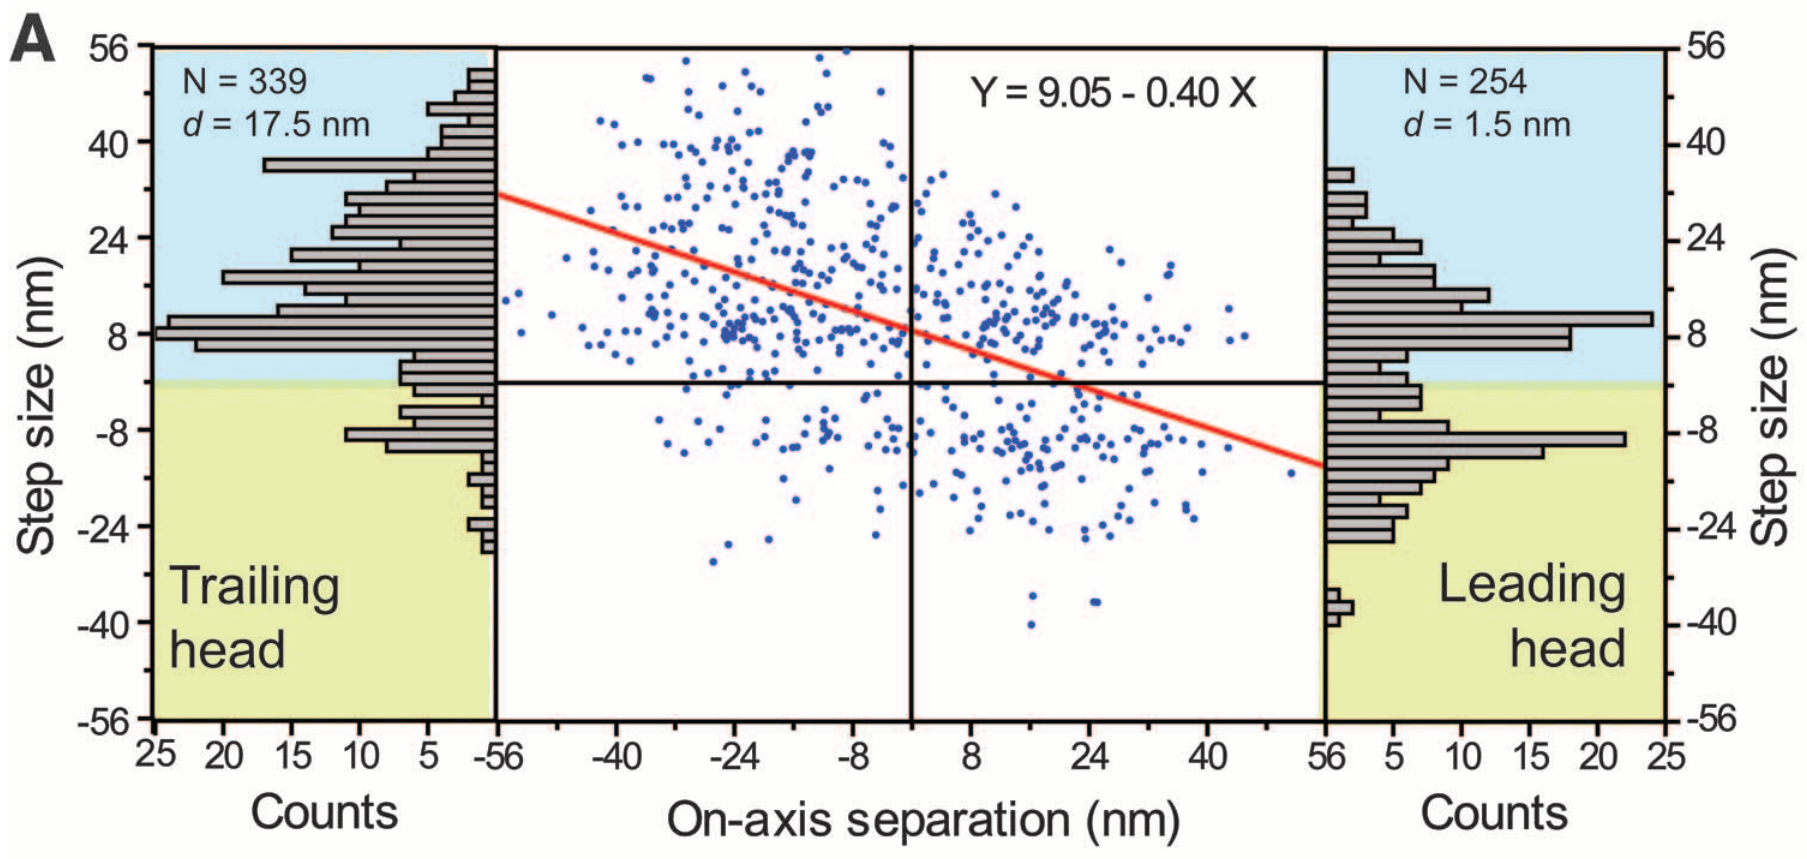
\includegraphics[width=1\columnwidth]{Figures/Yildiz_stepping.png}
	\caption[Stepping Correlation]{\textbf{Stepping Correlation}  \cite{Dewitt2012} }
	\label{fig:YildizCorrelation}
\end{figure}




\section{Motivation}
\textit{Briefly write about the importance of dynein, how dynein is researched when studying neurological diseases, dynein stepping is understudied compared to other motor proteins, hard to model dynein because of random walking, there are almost no computational models of dynein that uses molecular dynamics, modelling dyenin can give us better understanding of why it moves the way it does, specific motivation for model: new research found that there is interhead coordination when stepping so maybe we can use that to base our model off of.}
\par

To bridge this gap, we propose a coarse-grained model of dynein that assumes a particle-rod structure for its various domains and uses Brownian motion to simulate the model’s behavior in physically realistic drag and diffusion conditions, while efficiently collecting a wide ensemble of statistics using Monte Carlo methods. We chose to use Brownian inspired motion to simulate dynein’s molecular dynamics in order to replicate dynein’s stochastic behavior under realistic conditions and produce its unpredictable stepping patterns observed from experiment. We call this process Brownian dynamics, as it replaces interactions the domains have with solvent molecules with a stochastic force and allows us to simulate large time scales compared to other molecular dynamics simulation. Likewise, Monte Carlo methods will allow us to visualize dynein as a system and associate its possible configurations as states. With our simulation following these methods, we can generate an ensemble of statistics and compare measured quantities with experiment. We intend to use this model to reproduce experimental measures and help verify existing understandings concerning the properties of dynein’s stepping mechanism. One of which being a question regarding dynein’s inter-step correlation. 